\chapter{Rete neurale} \label{chp:reteNeurale}
La precedente fase di analisi ha permesso di acquisire informazioni utili sulla
struttura del dataset e di conseguenza permettere la selezione di un modello
adatto a svolgere il compito di classificazione.

In questo capitolo verrà presentata la rete neurale utilizzata per svolgere il
compito di classificazione. In particolare verrà presentata la struttura della
rete neurale, il processo di addestramento e i risultati ottenuti.

Prima di presentare nel dettaglio la rete neurale, risulta necessario specificare 
come sono stati preparati i dati per l'addestramento della rete neurale.
\section{Preparazione dei dati}
La prima operazione svolta sui dati è stata la standardizzazione dei dati, in 
questo modo i dati sono stati trasformati in modo tale che la loro media sia 0
e la loro deviazione standard sia 1. Questa operazione è stata eseguita per
garantire che la rete neurale non sia influenzata da valori di input con scale
diverse.

La seconda operazione svolta sui dati è stata la suddivisione del dataset in
training set e test set. Il training set è stato utilizzato per addestrare la
rete neurale, mentre il test set è stato utilizzato per valutare le prestazioni
della rete neurale. La suddivisione del dataset è stata effettuata in modo tale
che il training set contenesse il $80\%$ dei dati, mentre il test set contenesse
il $20\%$ dei dati.

La suddivisione dei dati è stata effettuata in modo da mantenere la stessa 
percentuale di dati positivi e negativi in entrambi i set. Questa operazione è
stata effettuata per evitare che la rete neurale sia addestrata su un dataset
sbilanciato.
\section{Struttura della rete neurale}
La rete neurale utilizzata per svolgere il compito di classificazione è una rete
neurale feedforward. La struttura di questa rete neurale è stata definita in
base ai risultati ottenuti dalla fase di analisi e attraverso un processo di grid
search.

In particolare, dalla fase di analisi è stato selezionato un sottoinsieme di
feature le quali sono state utilizzate come input della rete neurale. Questo 
sottoinsieme è composto da 5 elementi, il che ha permesso di definire la struttura 
del layer di input della rete neurale. Questo primo strato è composto da 5 neuroni,
in cui la funzione di attivazione, come la struttura interna della rete, è stata
definita attraverso un processo di grid search.

Nello specifico, il processo di grid search ha permesso di valutare le prestazioni
della rete neurale al variare della funzione di attivazione, del numero di layer
nascosti e del numero di neuroni per ogni layer nascosto. La ricerca della 
combinazione migliore di questi iperparametri è stata effettuata attraverso una
cross validation a 5 fold, prendendo in considerazione solamente i dati del
training set.

Visti i risultati ottenuti nella fase di analisi e la volontà di mantenere i 
tempi di addestramento bassi, si è scelto di mantenere una struttura di dimensioni 
ridotte per la rete neurale, in modo tale da evitare l'overfitting. Per questo
motivo, l'operazione di grid search è stata effettuata prendendo in considerazione
un numero di neuroni per layer nascosto tra 5, 10, 50, mentre il numero di
layer nascosti è stato valutato tra 1 e 2. Mentre, per quanto riguarda la funzione 
di attivazione, sono state valutate le seguenti funzioni di attivazione: 
\textit{relu}, \textit{leaky relu} e \textit{sigmoid}.

\begin{figure}[!ht]
    \centering
    \begin{subfigure}[b]{0.3\textwidth}
        \centering
        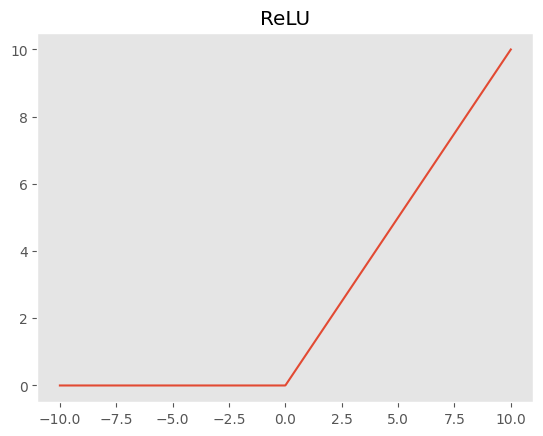
\includegraphics[width=\textwidth]{img/rete/relu.png}
        \caption{ReLU}
        \label{fig:relu}
    \end{subfigure}
    \hfill
    \begin{subfigure}[b]{0.3\textwidth}
        \centering
        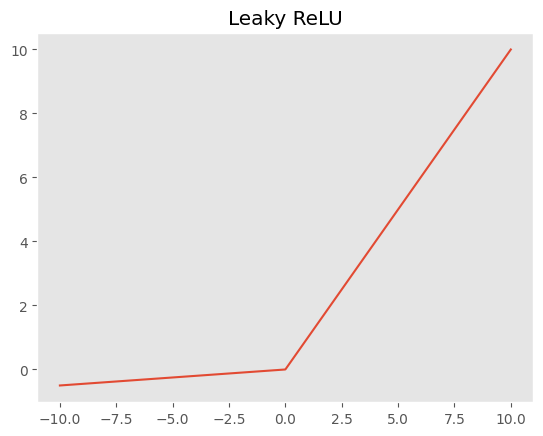
\includegraphics[width=\textwidth]{img/rete/leaky_relu.png}
        \caption{Leaky ReLU}
        \label{fig:leaky-relu}
    \end{subfigure}
    \hfill
    \begin{subfigure}[b]{0.3\textwidth}
        \centering
        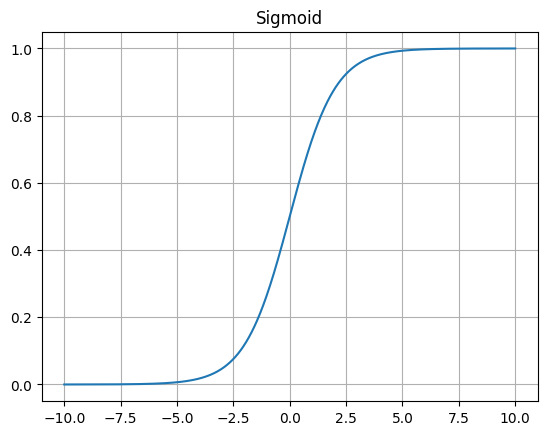
\includegraphics[width=\textwidth]{img/rete/sigmoid.png}
        \caption{Sigmoide}
        \label{fig:sigmoid}
    \end{subfigure}
       \caption{Funzioni di attivazione utilizzate nella fase di grid search}
       \label{fig:}
\end{figure}

I risultati ottenuti da questo processo di grid search hanno permesso di definire
la struttura della rete neurale. In particolare, la rete neurale è composta da:
%% TODO: definire la struttura della rete neurale

Per concludere la descrizione della struttura della rete neurale, è necessario
specificare come è composto l'ultimo layer, ovvero quello di output. Vista la  
natura del problema di classificazione, il layer di output è composto da un solo
neurone, in cui la funzione di attivazione è la funzione sigmoide. Questa scelta
è dovuta al fatto che tale funzione restituisce un valore compreso tra 0
e 1, il che permette di interpretare l'output della rete neurale come la
probabilità che l'input appartenga alla classe positiva.
\begin{equation}
    \sigma(x) = \frac{1}{1 + e^{-x}}
\end{equation}

Oltre alla ricerca
\section{Addestramento della rete neurale}
Definita la struttura della rete neurale, si è passati alla fase di addestramento
di questa. In questa fase è stato necessario definire la funzione di perdita,
l'algoritmo di ottimizzazione, il numero di epoche e la dimensione del batch.

Per quanto riguarda la funzione di perdita, è stata scelta la \textit{binary
    crossentropy} in quanto è una funzione di perdita adatta a problemi di
classificazione binaria. La scelta di questa funzione di perdita è dovuta alla 
natura del problema di classificazione che si vuole risolvere.

Gli altri iperparametri sono stati scelti attraverso un processo di grid search, 
nel quale sono state valutate le prestazioni della rete neurale al variare di
questi iperparametri. 

Questa fase di grid search è stata effettuando una cross validation a 5 fold,
prendendo in considerazione solamente i dati del training set. Durante le varie
iterazioni della cross validation, sono stati registrati i valori di accuratezza
e tempo di addestramento della rete neurale.

Queste informazioni sono state utilizzate per scegliere i valori degli iperparametri
che hanno permesso di ottenere i migliori risultati.

Per all'algoritmo di ottimizzazione il confronto è stato eseguito tra 
\textit{Adam} e \textit{SGD}, mentre per il numero di epoche e la dimensione
del batch sono stati valutati i valori 100, 300 per il numero di epoche e 50, 
100, 300 per la dimensione del batch.

% TODO: specificare i valori degli iperparametri scelti
\section{Risultati}
Il modello addestrato in precedenza è stato valutato sui dati che compongono il
test set. In particolare sono state valutate le seguenti metriche: accuratezza,
precisione, richiamo e F1 score. Oltre al calcolo di queste metriche, si è 
deciso di realizzare la curva ROC per il modello e di rappresentare la matrice
di confusione.

Prima di presentare i risultati ottenuti, è necessario specificare che essendo 
il dataset riferito a un ambito medico, si è deciso di aggiustare il valore di
threshold per la predizione del modello. In particolare, il valore di threshold
è stato impostato a $0.3$, in modo tale da ridurre il numero di falsi negativi.

Fatta questa precisazione, si può procedere con la presentazione dei risultati
ottenuti. In particolare, nella tabella \ref{tab:risultatiReteNeurale} sono
presentati i risultati ottenuti dal modello addestrato.

\begin{table}[ht]
    \centering
    \begin{tabular}{|c|c|}
        \hline
        \textbf{Metrica} & \textbf{Valore} \\
        \hline
        Accuratezza & ?? \\
        \hline
        Precisione & ?? \\
        \hline
        Richiamo & ?? \\
        \hline
        F1 score & ?? \\
        \hline
    \end{tabular}
    \caption{Risultati ottenuti dal modello addestrato}
    \label{tab:risultatiReteNeurale}
\end{table}

I risultati ottenuti sono giustificati dal fatto che le due classi sono linearmente
separabili.

% Lo facciamo alla fine? \section{Confronto con il percettrone}